\hfill
\begin{figure}[htbp]
\begin{center}
\resizebox{0.6\linewidth}{!}{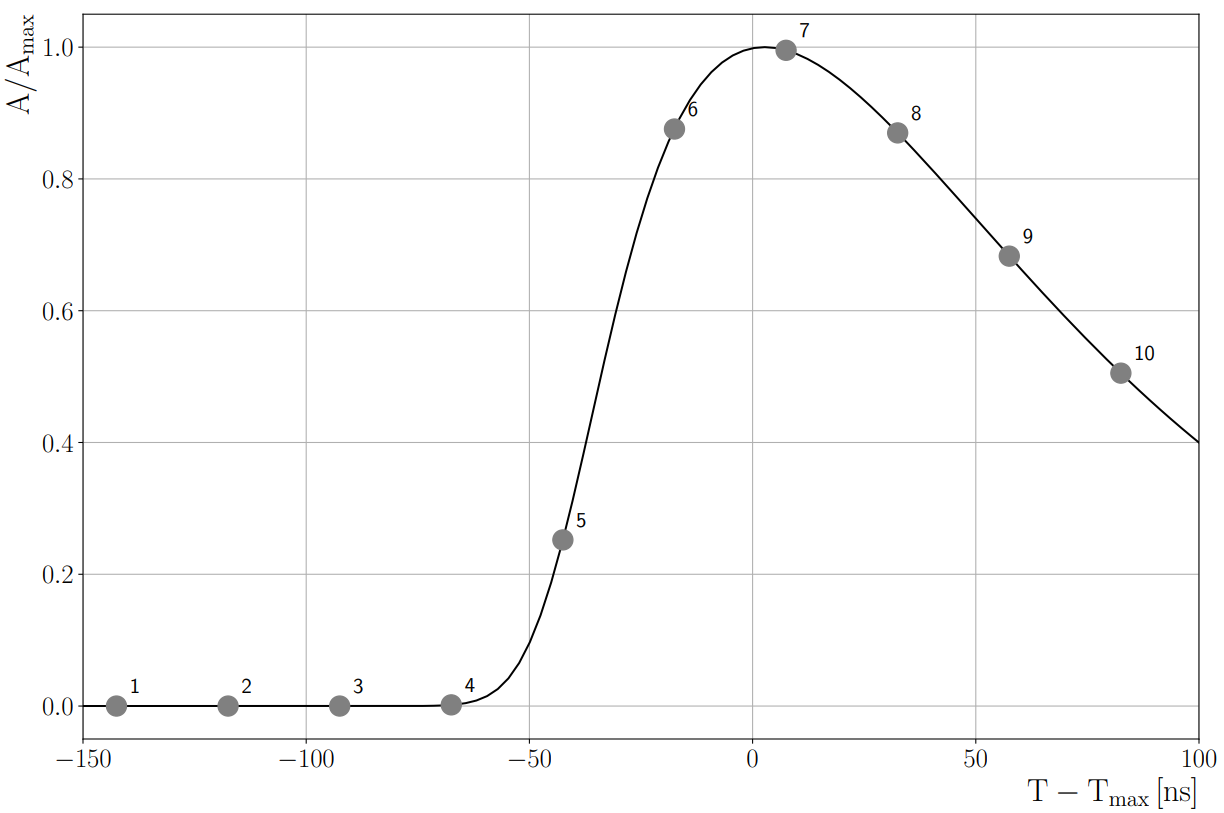
\includegraphics{fig/sec_reco/pulse_template.png}}
\caption{The typical pulse shape measured in the ECAL, as a function of the difference between the time (T) of the ADC sample and the time (Tmax) of the maximum of the pulse and the amplitude of the pulse (A) normalized by the maximum amplitude of the pulse (A$_{max}$).  The dots indicate ten discrete samples of the pulse as taken from a single event with the pedestal subtracted.}
\label{tec_pulseshape_ap}
\end{center}
\end{figure}

\hfill
\begin{figure}[htbp]
\begin{center}
\resizebox{0.6\linewidth}{!}{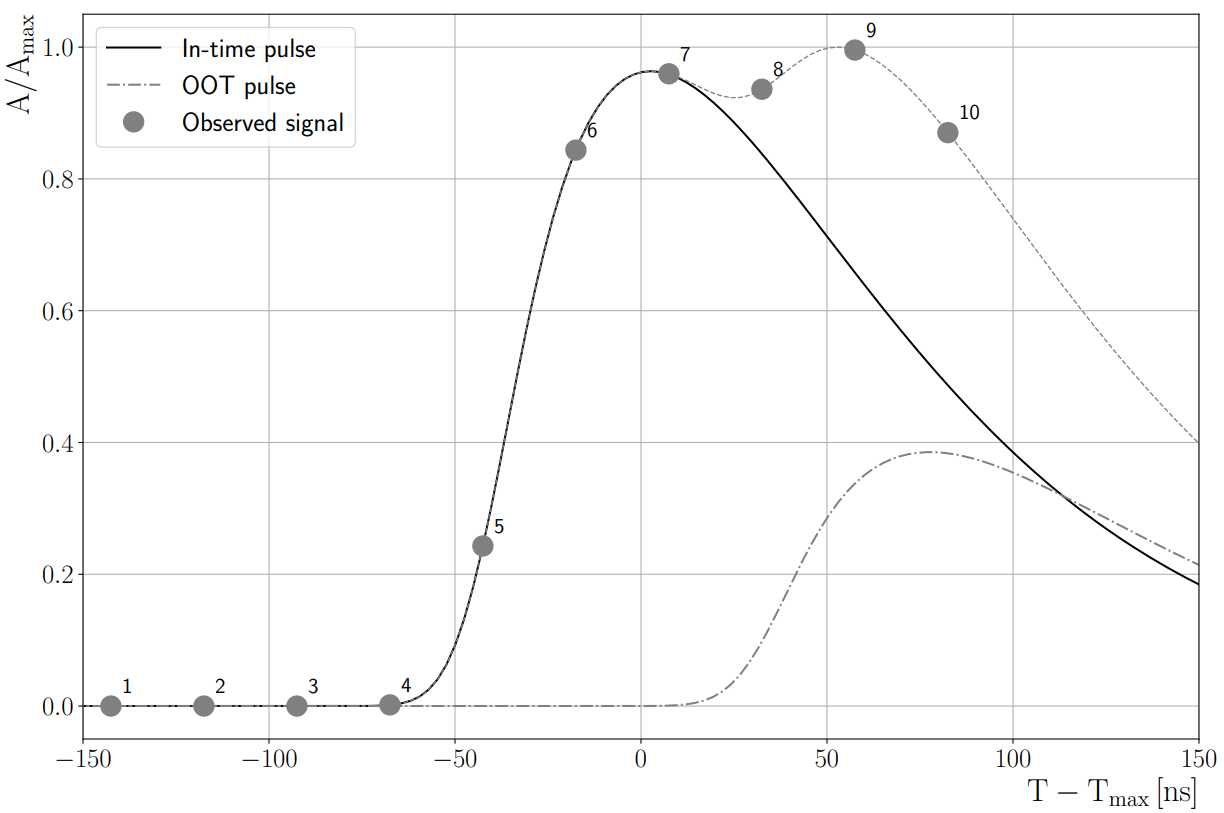
\includegraphics{fig/sec_reco/two_pulses.png}}
\caption{The fitted pulse for a simulated event with twenty average pileup events and 25 ns bunch spacing as a function of the difference between the time (T) of the ADC sample and the time (Tmax) of the maximum of the pulse and the amplitude of the pulse (A) normalized by the maximum amplitude of the pulse (A$_{max}$). The dots represent the 10 discrete samples of the measured pulse shape (dashed line) that is a superposition of an in-time pulse (solid line) and an OOT pulse (dashed line).
%Note that the samples are numbered starting at 0 instead of 1. 
}
\label{tec_multifit2_ap}
\end{center}
\end{figure}

\begin{figure}[htbp]
\begin{center}
\resizebox{0.75\linewidth}{!}{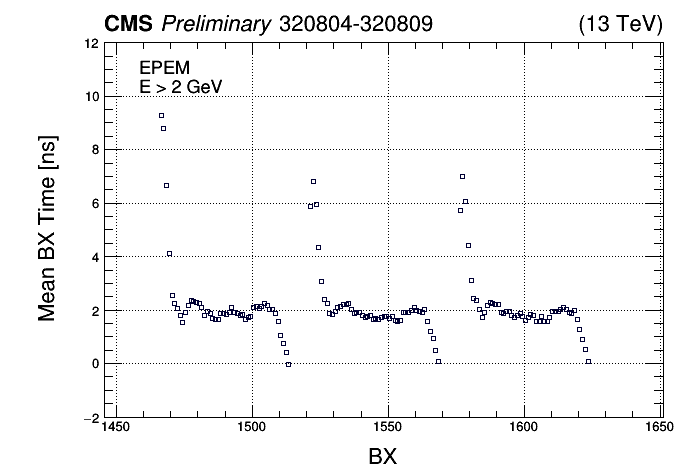
\includegraphics{fig/sec_motive/tr_lhc_18A_ratio2_note_05112021122552.png}}
\caption{The dependence of the rechit time on the position of a BX in a train of filled buckets. The mean of all the rechit times in a single BX are plotted with respect to the BX position of that BX. This plot demonstrates that the rechit time is highly dependent on the number of filled buckets before and after its BX position and biases the rechit time for rechits in the body of the train of filled buckets.}
\label{tam_timeresBX_ap}
\end{center}
\end{figure}

 \begin{figure}[htbp]
\begin{center}
\resizebox{0.75\linewidth}{!}{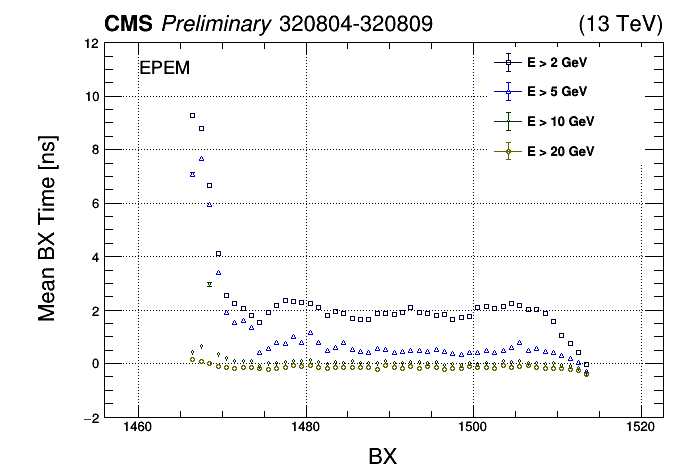
\includegraphics{fig/sec_motive/tr_lhc_18A_ratioall_note_05112021123825.png}}
\caption{The energy dependence of the rechit time on the position of a BX in a train of filled buckets. The mean of all the rechit times for all rechits with specified minimum energy in a single BX are plotted with respect to the BX position of that BX. The effect of OOT pileup on the mean rechit time is shown to be strongly dependent on the rechit energy.}
\label{trianedep_ap}
\end{center}
\end{figure}

\begin{figure}[!htbp]
\begin{center}
\resizebox{0.75\linewidth}{!}{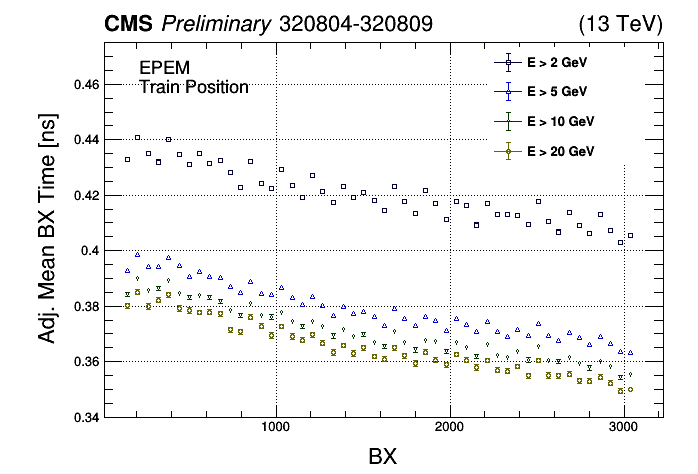
\includegraphics{fig/sec_motive/tr_lhc_18A_ratioall_stp_note_23112021155939.png}}
\caption{The energy dependence of the mean rechit time by BX is shown for all BX positions. The BX positions are grouped in bins of 50 BXs to better resolve the effects at this scale. The mean time is also seen to have an overall dependence on the BX position in the beam cycle. This dependence on BX position was attributed to the drift in the RF phase during the beam cycle.}
\label{tam_timeresbxe_ap}
\end{center}
\end{figure}

\begin{figure}[htbp]
\begin{center}
%\resizebox{0.48\linewidth}{!}{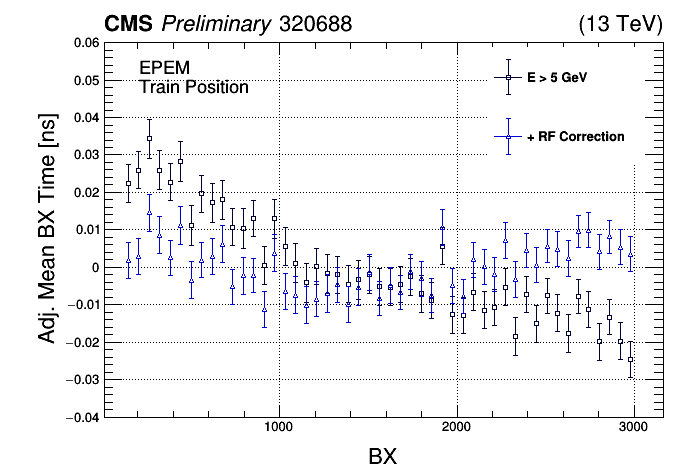
\includegraphics{fig/sec_motive/tr_lhc_18A_rfc_stp_note_23112021145355.png}}
\resizebox{0.75\linewidth}{!}{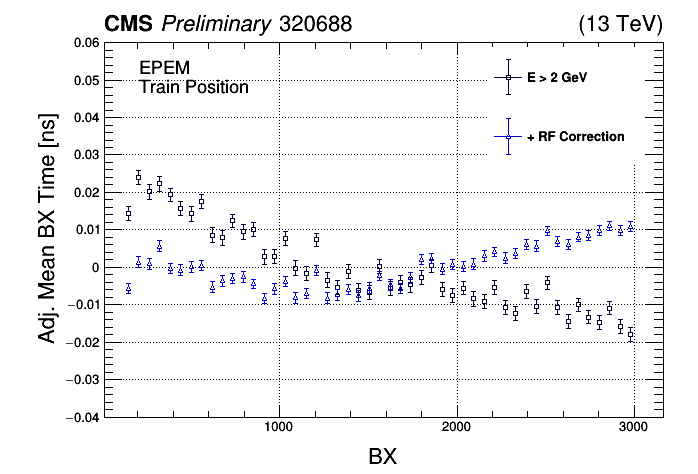
\includegraphics{fig/sec_motive/tr_lhc_18A_rfc_stp_note_23112021150000.png}}
\caption{The mean rechit time of all rechits in the BXs of a train of filled buckets in which the mean rechit times for all rechits with an energy greater than 2 GeV, adjusted so that the mean rechit time by BX when averaged over all BX positions is zero, as a function of the position of the train in the beam cycle. The first set of data points (squares) shows the dependence of the rechit time on the RF phase drift during the beam cycle. The RF phase corrected data points (triangles) have a correction for the RF Phase drift applied in the time reconstruction. The RF phase correction is shown to have a negligible impact on the time reconstruction.}
\label{tam_lhcrhphasecor_ap}
\end{center}
\end{figure}

\hfill
\begin{figure}[htbp]
\begin{center}
\resizebox{0.32\linewidth}{!}{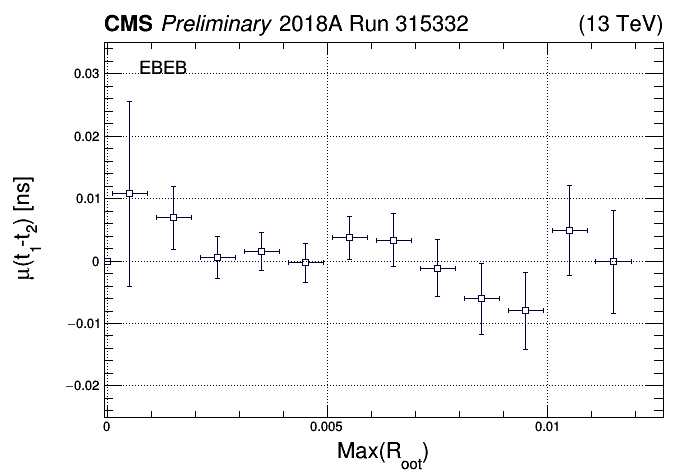
\includegraphics{fig/sec_motive/tr_hl_ootAmpMax_mean_17112021154025.png}}
\resizebox{0.32\linewidth}{!}{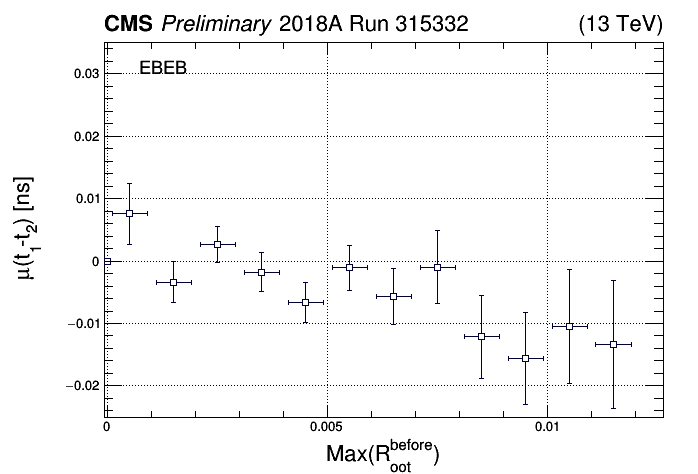
\includegraphics{fig/sec_motive/tr_hl_ootAmpMBfr_mean_17112021155948.png}}
\resizebox{0.32\linewidth}{!}{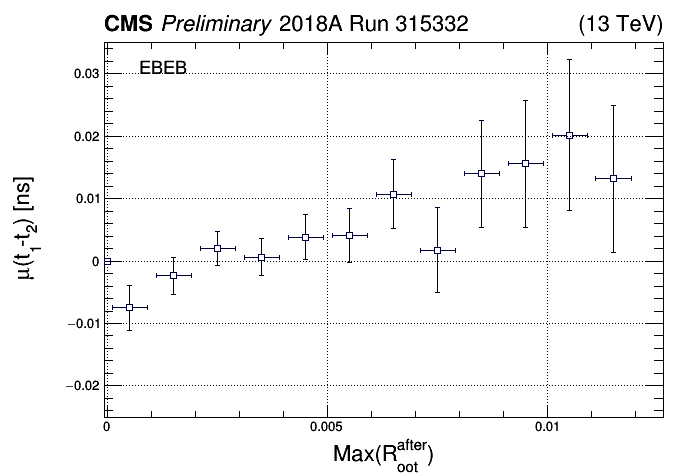
\includegraphics{fig/sec_motive/tr_hl_ootAmpMAft_mean_17112021155914.png}}
\resizebox{0.32\linewidth}{!}{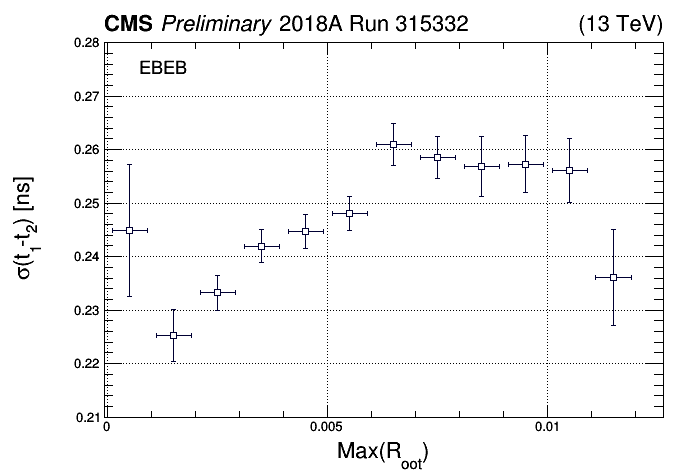
\includegraphics{fig/sec_motive/tr_hl_ootAmpMax_sigma_17112021150325.png}}
\resizebox{0.32\linewidth}{!}{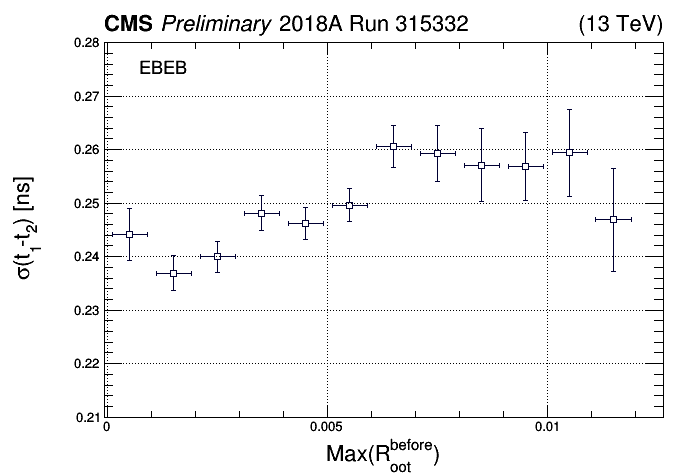
\includegraphics{fig/sec_motive/tr_hl_ootAmpMBfr_sigma_17112021151827.png}}
\resizebox{0.32\linewidth}{!}{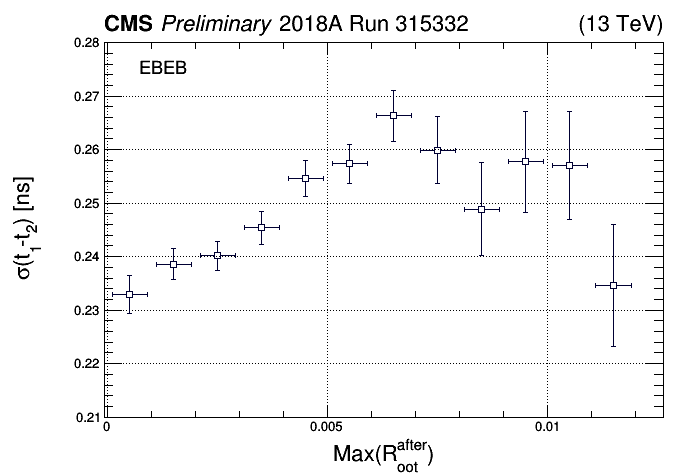
\includegraphics{fig/sec_motive/tr_hl_ootAmpMAft_sigma_17112021151937.png}}
\caption{Mean ($\mu$, top) and width ($\sigma$, bottom) of the difference in the reconstructed times for the seed crystal of an EG candidate and an adjacent crystal to the seed crystal are shown as a function of the three cases of the ratio, $R_{oot}$, of the nominal amplitude to the maximum OOT amplitude. Max$(R_{oot})$, the largest ratio found amongst all nine of the OOT amplitudes, is shown on the left. Max$(R_{oot}^{before})$, the largest ratio found amongst the five OOT amplitudes before the nominal amplitude, is shown in the middle. And Max$(R_{oot}^{after})$, the largest ratio found amongst the four OOT amplitudes after the nominal amplitude, is shown on the right. The plots for $\mu$ indicate that the mean of the time difference is biased in the direction of the larger values of $R_{oot}$. The plots for $\sigma$ indicate that in all cases the width of the distribution increases with larger values of $R_{oot}$.}
\label{tam_ootampbias_ap}
\end{center}
\end{figure}

\begin{figure}[htbp]
\begin{center}
\resizebox{0.75\linewidth}{!}{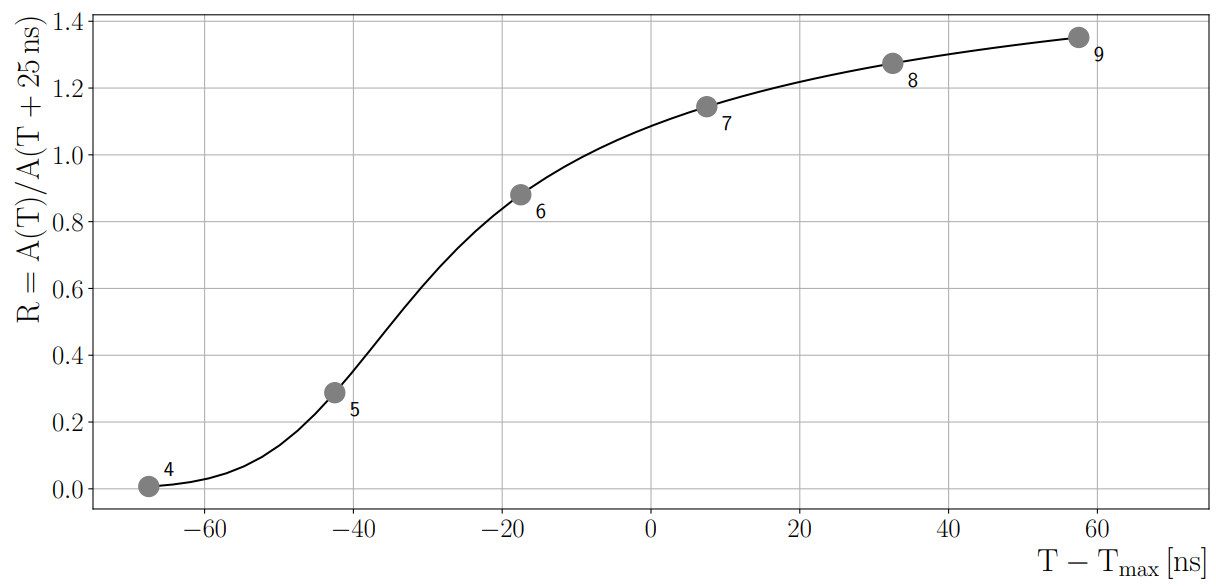
\includegraphics{fig/sec_reco/ratio_tvR_mod.png}}
\caption{The ratio, $R$, of two consecutively measured amplitudes, $A(T)$ and $A(T+25 ns)$, as a function of the time difference $T-T_{max}$, where $T_{max}$ is the time when the pulse reaches its maximum value. The first three amplitudes, $A(1)$, $A(2)$, and $A(3)$, typically used to measure the pedestals values for the pulse, are not used. The rechit time is determined from the weighted averages of three consecutive value of $R(A(4)/A(5))$ through $R(A(7)/A(8))$.}
\label{tec_pulseratio_ap}
\end{center}
\end{figure}

\begin{figure}[htbp]
\begin{center}
\resizebox{0.95\linewidth}{!}{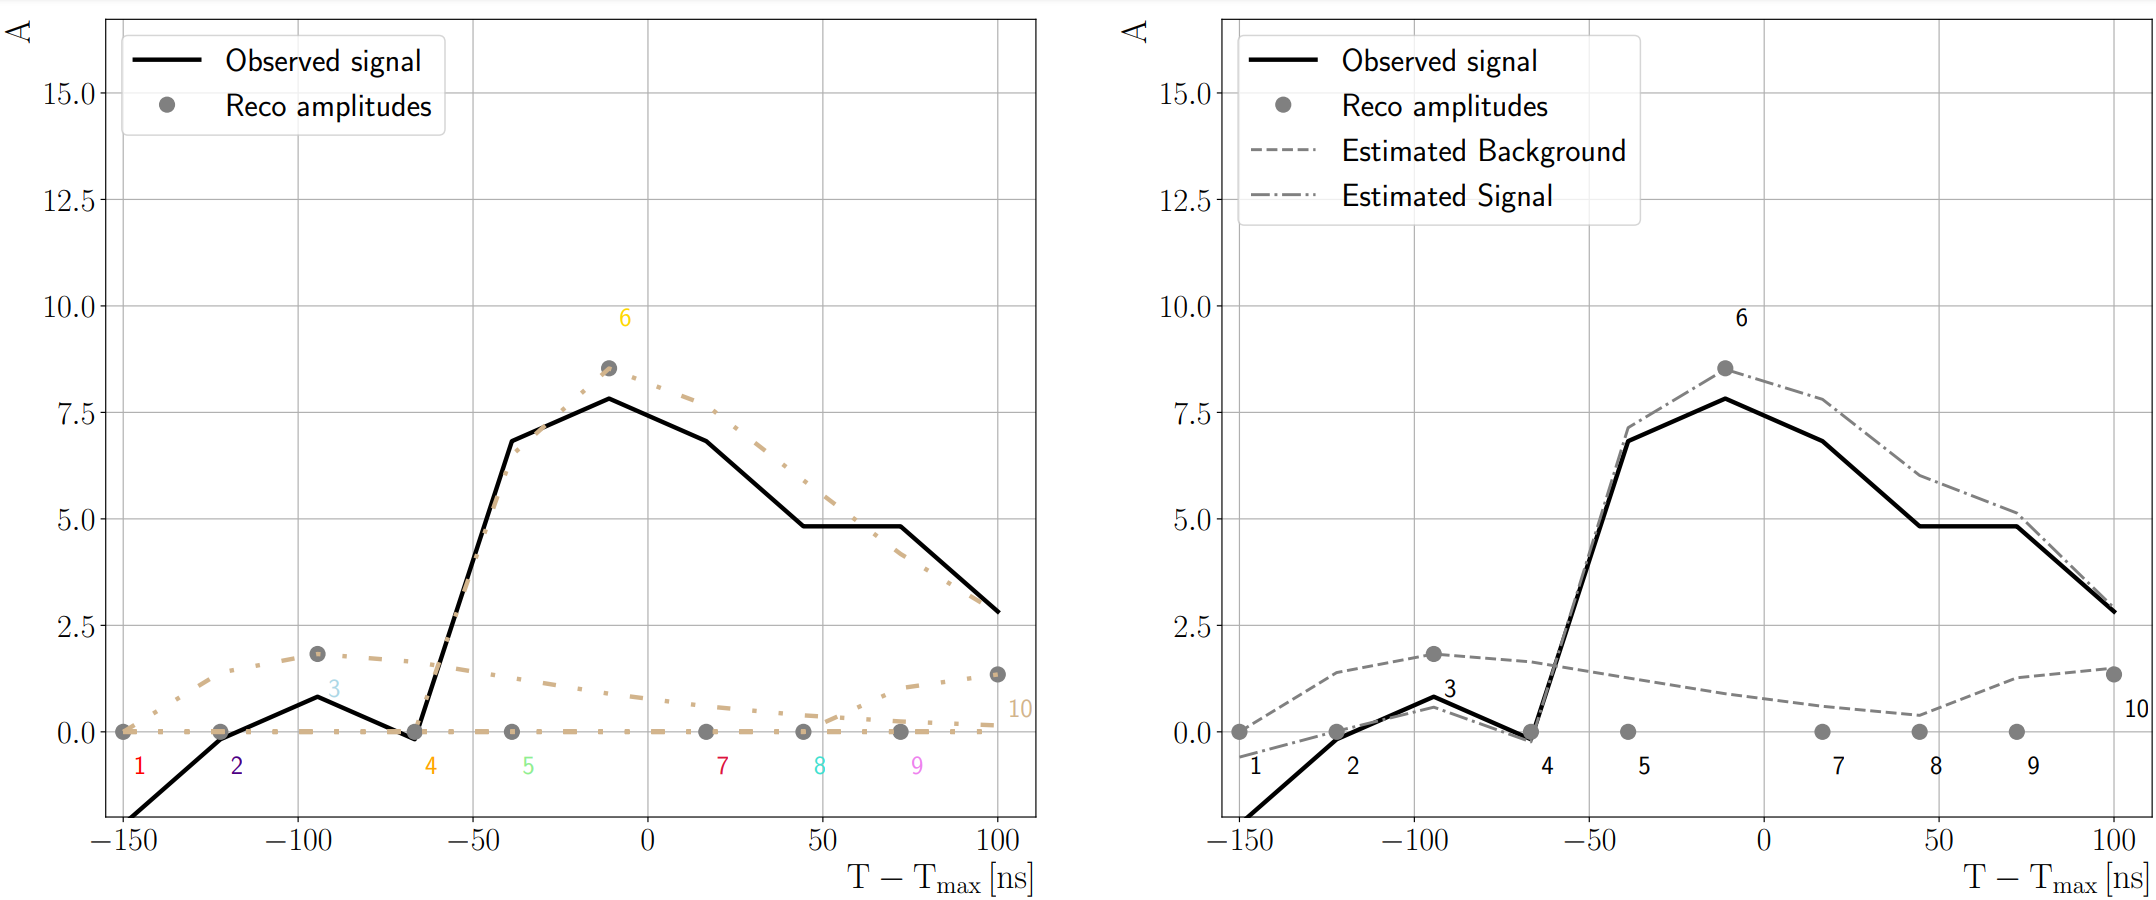
\includegraphics{fig/sec_algos/fOOT_reco_a2.png}}
%\resizebox{0.65\linewidth}{!}{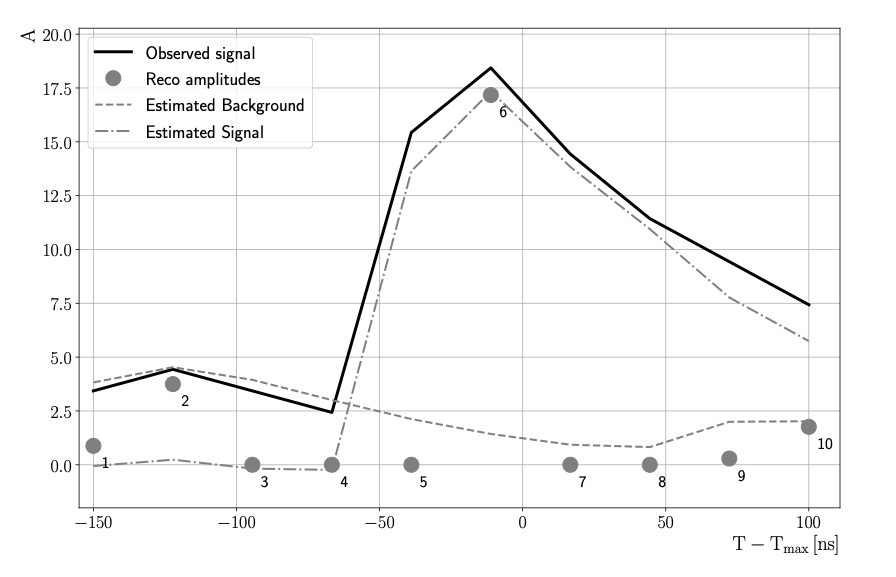
\includegraphics{fig/sec_reco/mfit_pulses_sing.png}}
\caption{An illustration of the OOT amplitude correction for the proposed time reconstruction method. In both plots the black line is the measured signal, $H(bx)$ and the black dots are the reconstructed amplitudes from the multi-fit, $A^{mf}_{i}$. In the plot on the left the double doted dashed lines are the nine OOT pulses, $F^{OOT}_{i}(A^{mf}_{i},t)$, including the nominal, or in-time, pulse given by amplitude 6, that are all reconstructed from $A^{mf}_{i}$. In the plot on the right the dashed line is the background pulse shape, $F_{bg}(bx,t)$, that is the linear combination of the OOT amplitudes. The dotted dashed line is the recovered signal, $A^{sig}(bx,t)$, that is found by subtracting the background pulse shape from the measured signal.}
\label{tra_pulsereco_ap}
\end{center}
\end{figure}

\hfill
\begin{figure}[h!tbp]
\begin{center}
%\resizebox{0.5\textwidth}{!}{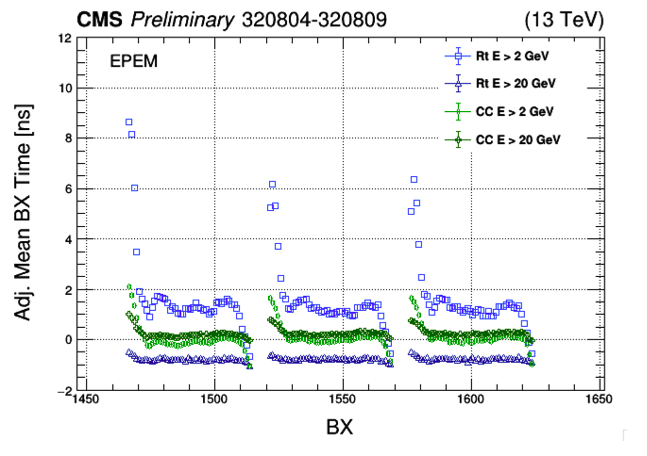
\includegraphics{fig/sec_results/lhc_cc_v_rt_plot.png}}
\resizebox{0.75\textwidth}{!}{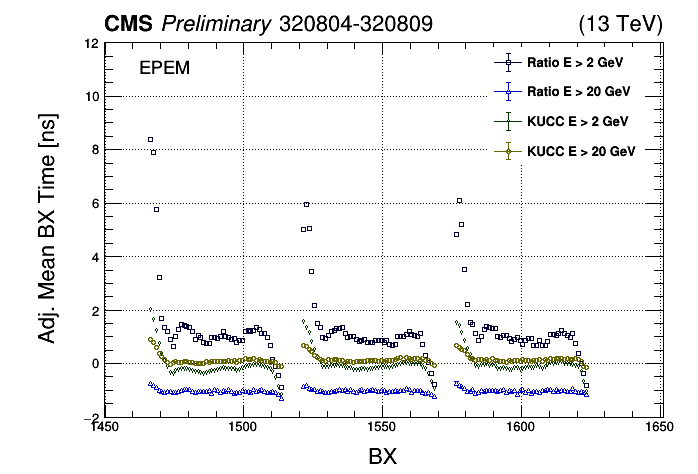
\includegraphics{fig/sec_results/tr_lhc_18A_v25_talk_30112021151421.png}}
\caption{Mean rechit time by BX, for rechits with a minimum of 2 GeV ( 20 GeV ) with both the ratio and KUCC reconstructions, for a typical trains of filled buckets is plotted in Runs 320804 through 320809 of EGamma Run2018D-22Jan2019-v2. The plotted values are adjusted so that the mean rechit time by BX when averaged over all BXs and energies is zero. The KUCC algorithm is shown to mitigate the impact of OOT-PU through the reduced dependence of the time on the BX position and to achieve a greatly reduced energy dependence.}
\label{cclhcplots1_ap}
\end{center}
\end{figure}

\hfill
\begin{figure}[h!tbp]
\begin{center}
%\resizebox{0.5\textwidth}{!}{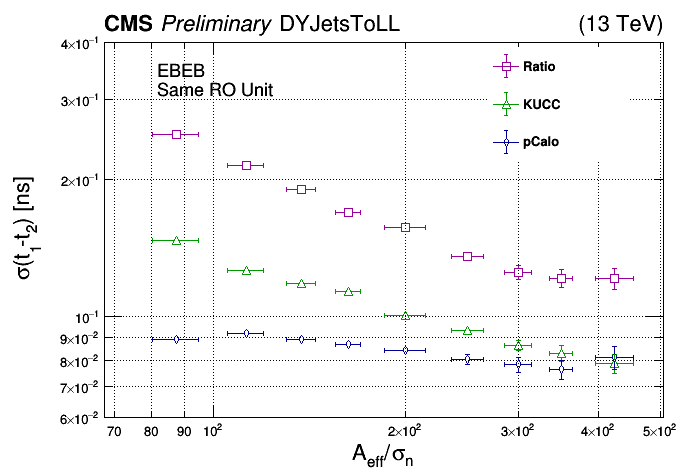
\includegraphics{fig/sec_gen/tr_mc_pc2_loc_plot_07122020164223.png}}
\resizebox{0.75\textwidth}{!}{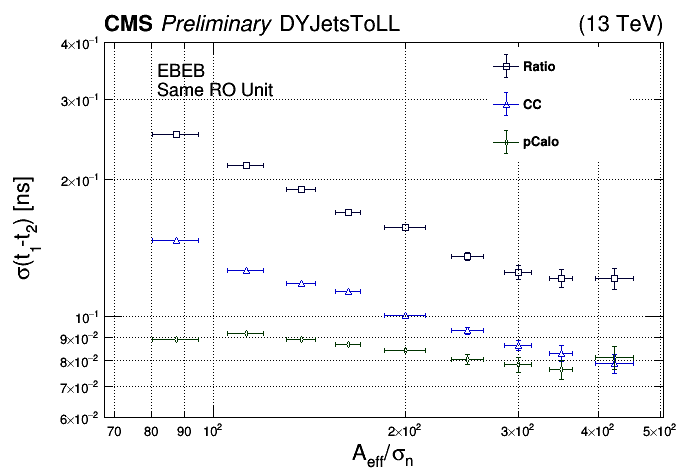
\includegraphics{fig/sec_gen/tr_mc_pc2_loc_plot_30112021153817.png}}
\caption{Same RO unit, single crystal resolutions for the ratio algorithm, the KUCC algorithm, and pCaloHit gen time produced with the DYJetsToLL\_M-50\_TuneCP5\_13TeV-madgraphMLM-pythia8 Monte Carlo dataset. The KUCC algorithm shows a much improved resolution compared to the ratio algorithm and approaches the pCaloHit gen time resolution at high energies.}
\label{pc_rt_cc_comp_ap}
\end{center}
\end{figure}

\begin{figure}[h!tbp]
\begin{center}
%\resizebox{0.33\textwidth}{!}{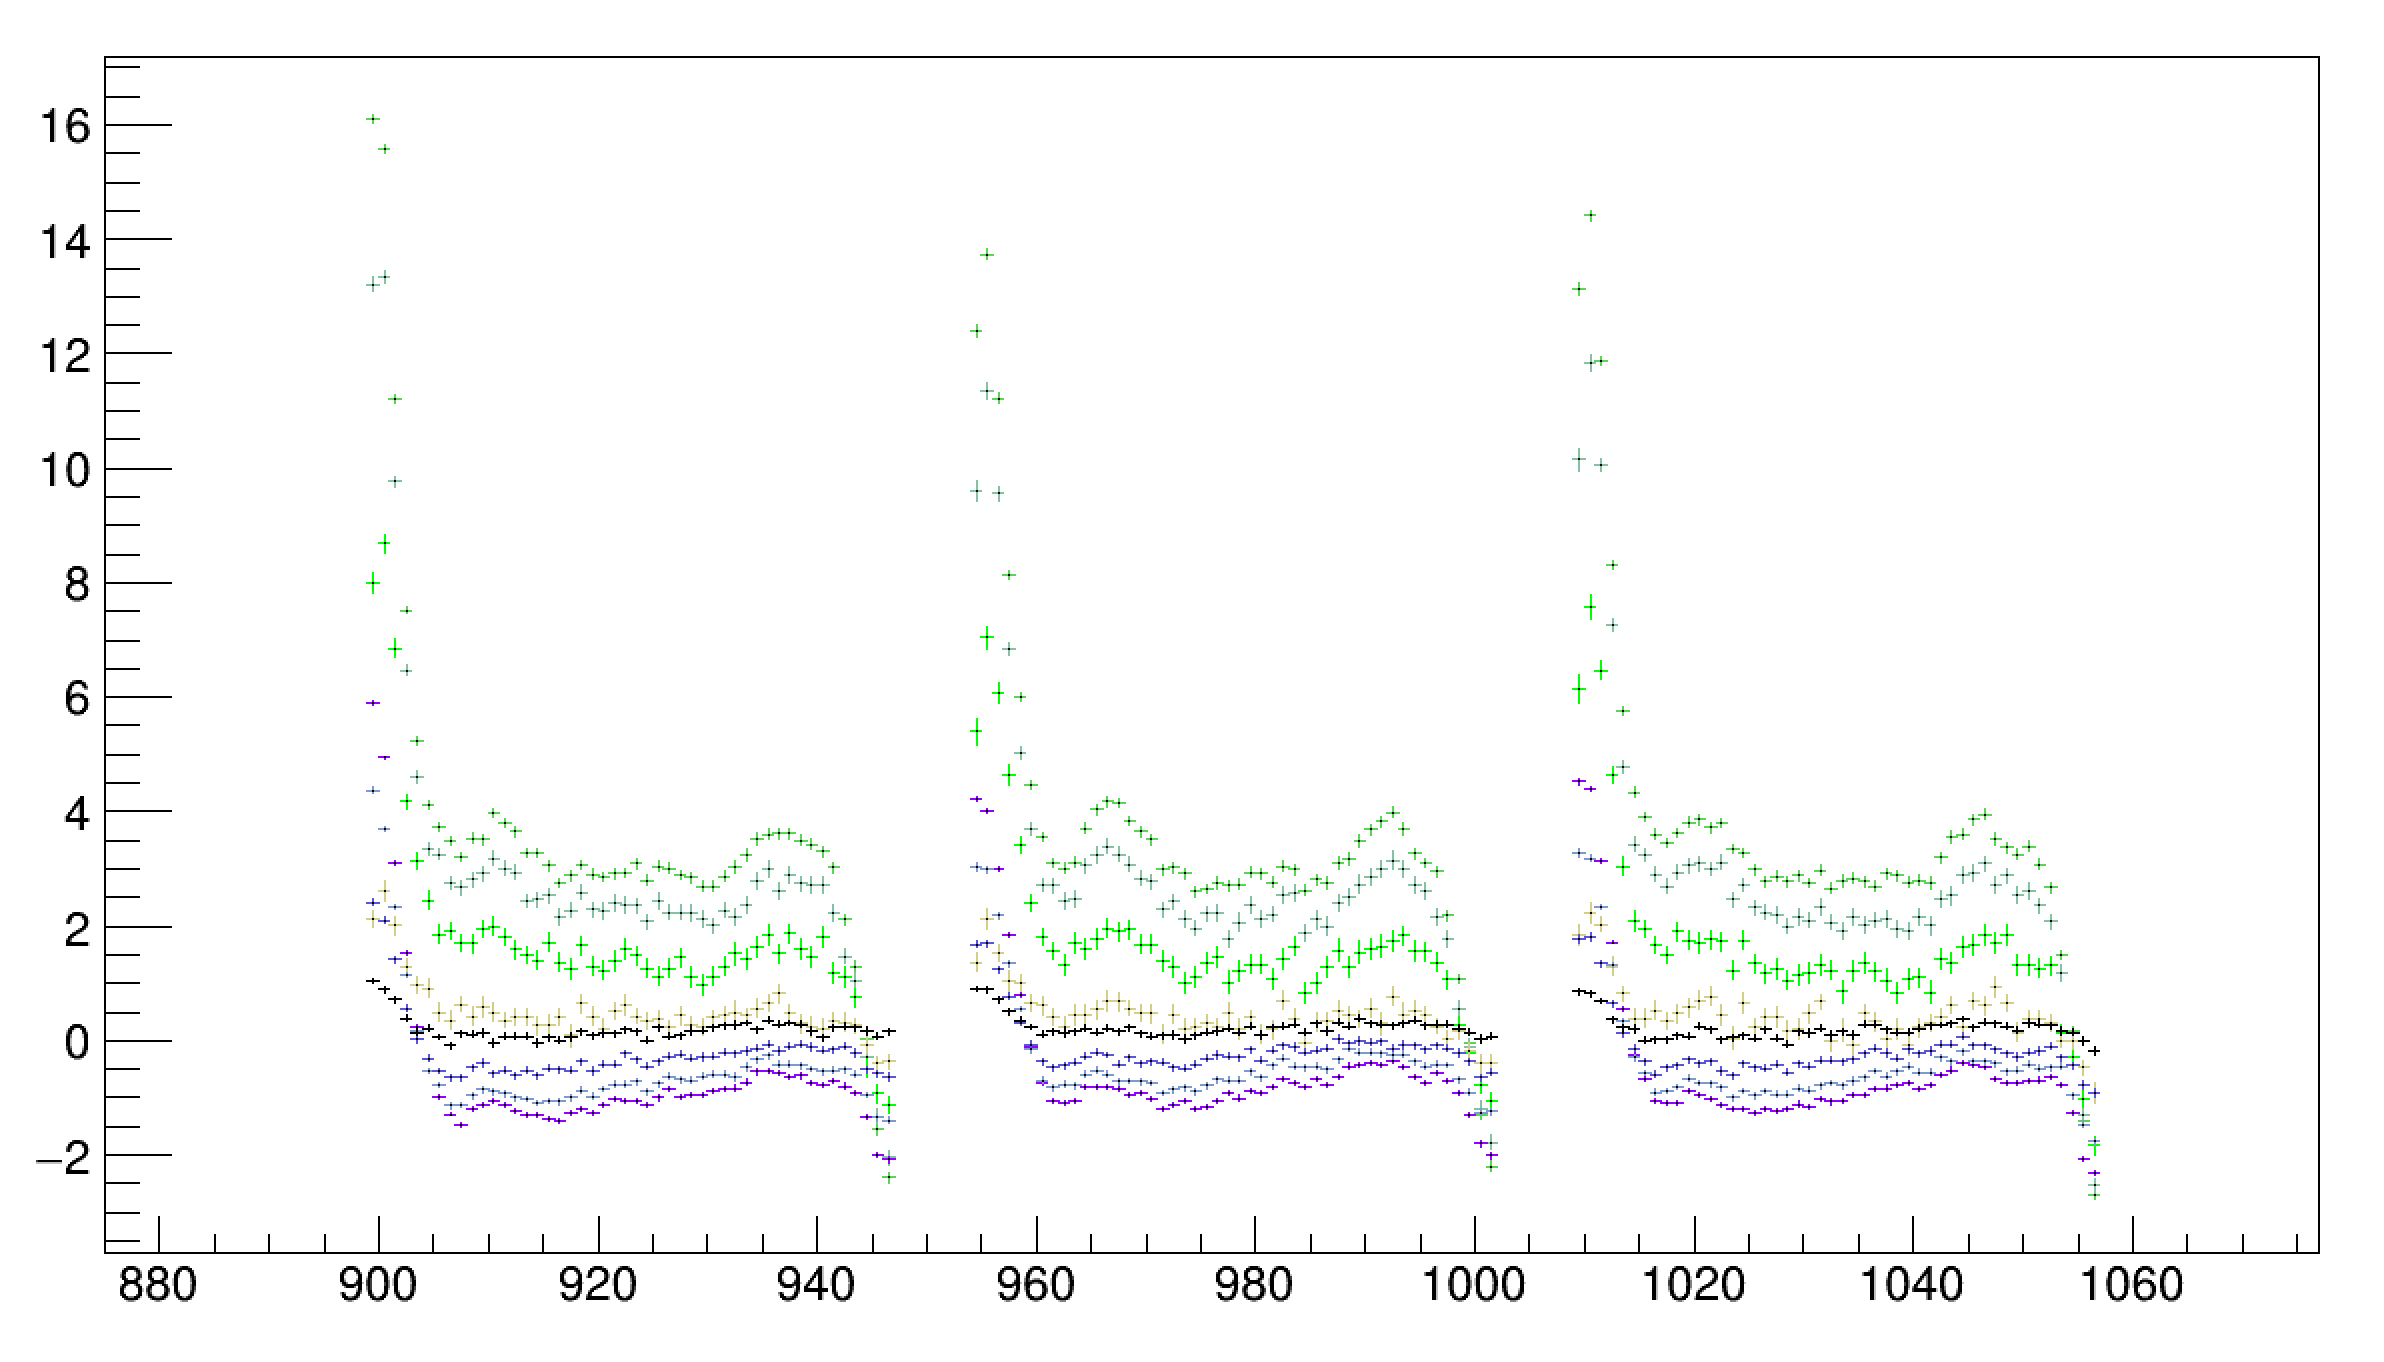
\includegraphics{fig/sec_results/full_lhc_info.png}}
%\resizebox{0.5\textwidth}{!}{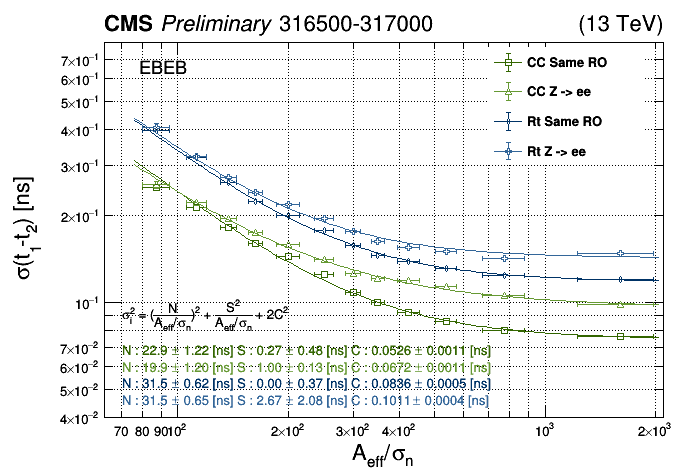
\includegraphics{fig/sec_results/tr_kucc_18As_v25_talk_17092021152333.png}}
\resizebox{0.75\textwidth}{!}{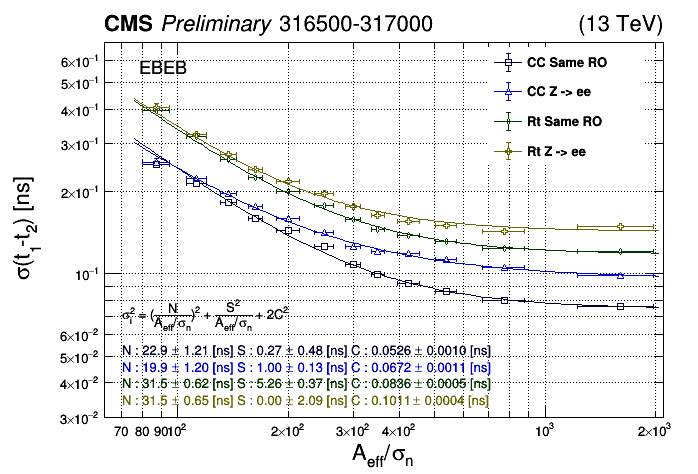
\includegraphics{fig/sec_results/tr_kucc_18As_v25_talk_30112021160215.png}}
\caption{Comparison of time Same RO and $Z\rightarrow e^{+}e^{-}$ resolution for KUCC and the ratio algorithms in run 316500 through run 317000 of the EGamma Run2018A-17Sep2018-v2 rereco. This plot shows that the KUCC algorithms achieves an improvement in the Same RO unit resolution of $\sim$30 ps and an $Z\rightarrow e^{+}e^{-}$ resolution improvement of $\sim$35 ps.}
\label{ccres_ap}
\end{center}
\end{figure}

